\documentclass{article}
\usepackage{amsmath}
\usepackage{graphicx}
\usepackage{array}
\usepackage{unicode-math}
\usepackage[UTF8]{ctex}
\usepackage[hidelinks]{hyperref}
\usepackage{gbt7714}
\usepackage{listings}
\usepackage{geometry}
\usepackage{xcolor}

\geometry{a4paper,left=2cm,right=2cm,top=2cm,bottom=2cm}

\lstset{
    %backgroundcolor=\color{red!50!green!50!blue!50},%代码块背景色为浅灰色
    rulesepcolor= \color{gray}, %代码块边框颜色
    breaklines=true,  %代码过长则换行
    numbers=left, %行号在左侧显示
    numberstyle= \small,%行号字体
    %keywordstyle= \color{blue},%关键字颜色
    commentstyle=\color{gray}, %注释颜色
    }

\begin{document}
\begin{figure}[!ht]
    \centering
    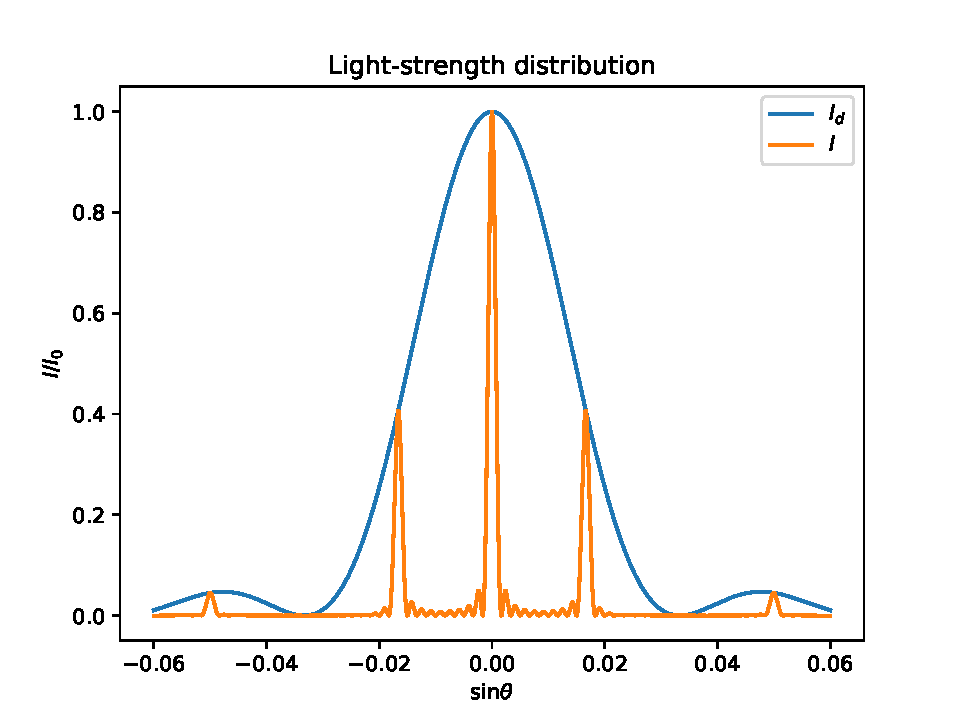
\includegraphics[width=15cm]{FRP.pdf}
\end{figure}

\begin{lstlisting}[language={python}]
import numpy as np
import matplotlib.pyplot as plt
from math import pi

Lambda = 0.5
d = 30
a = 15
n = 10
sintheta = np.linspace(-0.06, 0.06, 12000)
alpha = pi*a*sintheta/Lambda
beta = pi*d*sintheta/Lambda
id = (np.sin(alpha)/alpha)**2
id = id/max(id)
ii = (np.sin(n*beta)/np.sin(beta))**2
ii = ii/max(ii)
i = id*ii

plt.plot(sintheta, id, label="$I_d$")
plt.plot(sintheta, i, label="$I$")
plt.xlabel("$\sin{\\theta}$")
plt.ylabel("$I/I_0$")
plt.title("Light-strength distribution")
plt.legend()
plt.show()
\end{lstlisting}
\end{document}